\chapter{Curved Space and the Geometry of Cosmology}

These notes follow Leonard Susskind's third cosmology lecture closely. The preserved board frames from LazyingArt LLC and Video2Book are kept where they genuinely carry mathematical or diagrammatic evidence, but the transcript remains the primary source of order, emphasis, and interpretation. The lecture begins by loosening an assumption rather than proving a theorem. We have been acting as if space were flat; observation says that this is a very good approximation, but flatness is not a principle. So the right question is: if we keep the cosmological assumption of homogeneity and isotropy, what other geometries are possible? We first discuss space by itself. Only after that static story is in place do we return to spacetime and expansion.

\section{Why Cosmology Must Reopen Geometry}

We have not said much about geometry so far, and in particular we have not said much about spacetime geometry. Up to this point flat space has been the default background. But that default was a convenience, not a deduction. The lecture insists on this distinction. We do not know that space is flat. We know, rather, that if it is curved then its radius of curvature must be very large compared with the region we directly observe.

Once that point is made, the lecture narrows the possibilities in the characteristic Susskind way. We drop the assumption of flatness, but for the moment we retain homogeneity and isotropy. Homogeneity means that every observer sees the same local geometry. This one demand already throws away most curved spaces one can easily draw. A paraboloid is more curved near its tip than far away. A long ellipsoid is different at the poles and at the waist. A sphere with bumps, or even the Earth's surface with mountains and valleys taken seriously, is not homogeneous. Such spaces may be curved, but they are not good cosmological models if we want every point to be on the same footing.

So the question is not simply, ``What curved spaces exist?'' The question is, ``What curved spaces can be curved and still homogeneous?'' At first pass the lecture isolates three simply connected constant-curvature cases: flat space, positively curved spherical space, and negatively curved hyperbolic space. A later caveat will add the torus as a flat but multiply connected possibility. Before we get there, however, we need the real language of geometry, namely the metric.

\section{Metrics, Polar Coordinates, and the Unit Circle}

A space is specified by its metric, that is, by the squared distance between neighboring points. For ordinary flat three-dimensional space the opening example is
\begin{equation}
ds^2 = dx^2 + dy^2 + dz^2.
\end{equation}

\begin{figure}[htbp]
\centering

\includegraphics[width=0.74\textwidth]{lecture_03_figure_02.png}
\caption{Flat-space metric in Cartesian coordinates, as written on the board.}
\end{figure}

In two dimensions we would have simply
\begin{equation}
ds^2 = dx^2 + dy^2.
\end{equation}
To go from the plane to flat three-space we merely add the third orthogonal contribution \(dz^2\). That simplicity is not the point. The point is that once the metric is known, the geometry is known.

The lecture now changes coordinates, and this is the first important pedagogical pivot. We are not changing coordinates because polar coordinates are more elegant. We are changing coordinates because cosmology is observer-centered. We look out into the sky by angles. In a two-dimensional universe our entire visual field would literally be angular. So let us introduce a radial distance \(r\) and an angle \(\theta\). The flat metric on the plane becomes
\begin{equation}
ds^2 = dr^2 + r^2 d\theta^2.
\end{equation}
The board itself writes only \(d\Omega^2\), with no visible subscript, but the transcript makes clear what is intended: the angular factor is the metric of the unit circle. We therefore standardize the notation as
\begin{equation}
d\Omega_1^2 = d\theta^2,
\qquad\text{so that}\qquad
ds^2 = dr^2 + r^2 d\Omega_1^2.
\end{equation}

\begin{figure}[htbp]
\centering

\includegraphics[width=0.74\textwidth]{lecture_03_figure_03.png}
\caption{Flat space written in polar form; the board shows \(d\Omega^2\), which the lecture identifies with the metric of the unit circle.}
\end{figure}

\begin{figure}[htbp]
\centering
\begin{tikzpicture}[scale=1.2]
\draw[->] (-1.2,0)--(1.8,0);
\draw[->] (0,-1.2)--(0,1.8);
\draw[thick] (0,0)--(1.3,1.1);
\draw (0.7,0.7) node[above] {$r$};
\draw (0.58,0) arc (0:40:0.58);
\draw (0.8,0.22) node {$\theta$};
\end{tikzpicture}
\caption{A clean redraw of the polar-coordinate sketch that accompanies the metric \(ds^2 = dr^2 + r^2 d\Omega_1^2\).}
\end{figure}

The factor \(r^2\) is already telling us something geometrical. At fixed \(r\), a small angular interval \(d\theta\) corresponds to an arc length \(r\,d\theta\). Squaring that gives \(r^2 d\theta^2\). So the transverse part of the metric grows with \(r^2\). In other words, the circles around us get bigger and bigger linearly with distance.

\subsection{Question \& Answer}

Why does \(d\theta^2\) count as the metric of a circle?

Because on a unit circle the angular coordinate \(\theta\) is itself the intrinsic coordinate along the space. Two neighboring points separated by \(d\theta\) are separated by an arc length \(d\theta\), so the squared distance is \(d\theta^2\). Thus \(d\theta^2\) is already a metric before we place it inside the polar metric of the plane.

This is precisely where the lecture pauses over intrinsic geometry. If we insist on embedding the unit circle in a Euclidean plane, we may describe it by
\begin{equation}
x^2 + y^2 = 1.
\end{equation}
But that equation belongs to the embedding picture, not to the intrinsic metric alone. The deeper point is that the metric \(d\theta^2\) would remain the same even if we deformed the circle into a lopsided closed loop, provided equal increments of \(\theta\) still marked equal intrinsic distances along it. The space need not \emph{look} round in order to \emph{be} the same metric circle.

\begin{figure}[htbp]
\centering

\includegraphics[width=0.64\textwidth]{lecture_03_figure_04.png}
\caption{A round unit circle and a deformed but metrically equivalent closed loop.}
\end{figure}

\begin{figure}[htbp]
\centering
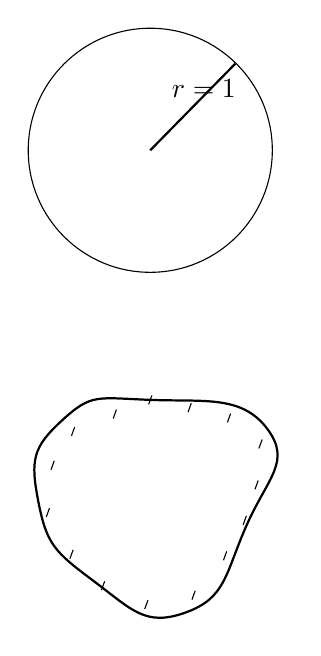
\begin{tikzpicture}[scale=1.0]
\draw (0,0) circle (1.55);
\draw[thick] (0,0)--(1.08,1.1);
\draw (0.68,0.78) node {$r=1$};

\begin{scope}[yshift=-4.35cm]
\draw[thick]
plot[smooth cycle, tension=0.95] coordinates
{(0,1.18) (1.48,0.82) (1.22,-0.42) (0.45,-1.52) (-0.72,-1.12) (-1.42,-0.12) (-1.12,0.92)};
\foreach \p in {(0,1.18),(0.5,1.08),(1.0,0.95),(1.4,0.62),(1.35,0.1),(1.2,-0.35),(0.95,-0.8),(0.55,-1.3),(-0.05,-1.42),(-0.6,-1.18),(-1.0,-0.78),(-1.3,-0.25),(-1.24,0.35),(-0.98,0.78),(-0.45,1.0)}{
\draw[rotate around={70:\p}] \p ++(-0.06,0) -- ++(0.12,0);
}
\end{scope}
\end{tikzpicture}
\caption{A schematic redraw of the lecture's point: ``circle'' is an intrinsic metric notion, not merely a Euclidean appearance.}
\end{figure}

Returning now to the plane, we may think of flat space as a nested sequence of circles around us. Each circle contributes the unit-circle metric multiplied by the square of its own radius. That is exactly what \(r^2 d\Omega_1^2\) means.

\section{Positive Curvature: The 2-Sphere and the 3-Sphere}

Now comes the lecture's main construction. A sphere is curved, but unlike a paraboloid or an ellipsoid it is still homogeneous. Every point on a sphere is the same as every other point. So let us try to build its metric in the same observer-centered way.

Imagine that we are two-dimensional astronomers living on a \(2\)-sphere. We stand at one point and look out. Nearby we see a small surrounding circle. A bit farther away we see a larger one. Farther still, a larger one again. But now the pattern differs from the flat plane. The circles do not keep growing forever. Their growth slows, reaches a maximum, and then reverses. Eventually the surrounding circles shrink back to a point at the antipode. And the lecture is very careful here: this is not a story about time. The circles grow and shrink as a function of \emph{distance} from us.

The notation shifts at this point and must be reset explicitly. On the unit \(2\)-sphere we use \(r\) not as an ordinary Euclidean radial distance but as the angular distance from our chosen origin. Thus
\[
0 \le r \le \pi.
\]
At \(r=0\) we are at our own point. At \(r=\pi/2\) we are at the equator. At \(r=\pi\) we are at the antipode. The surrounding circles have radius \(\sin r\), so the flat factor \(r^2\) is replaced by \(\sin^2 r\). The metric becomes
\begin{equation}
d\Omega_2^2 = dr^2 + \sin^2 r\, d\Omega_1^2
            = dr^2 + \sin^2 r\, d\theta^2.
\end{equation}
The lower board line is only partially visible in the preserved frame, but the transcript leaves no real ambiguity: the intended replacement is \(r^2 \mapsto \sin^2 r\).

\begin{figure}[htbp]
\centering

\includegraphics[width=0.82\textwidth]{lecture_03_figure_05.png}
\caption{The lecture's transition board from flat radial geometry to spherical radial geometry. The lower spherical line is only partially visible, but the transcript fixes the intended replacement \(r^2 \mapsto \sin^2 r\).}
\end{figure}

\begin{figure}[htbp]
\centering
\begin{tikzpicture}[scale=0.92]
\begin{scope}[xshift=-4.15cm]
\draw[->] (-1.7,0)--(1.9,0);
\draw[->] (0,-1.7)--(0,1.9);
\draw (0,0) circle (0.45);
\draw (0,0) circle (0.9);
\draw (0,0) circle (1.35);
\draw[thick] (0,0)--(1.45,1.2);
\draw (0.56,0.18) arc (18:40:0.63);
\draw (0.94,0.44) node {$\theta$};
\end{scope}

\begin{scope}[xshift=4.15cm]
\draw (0,0) circle (2.0);
\fill (0,-2.0) circle (1.5pt);
\fill (2.0,0) circle (1.5pt);
\fill (0,2.0) circle (1.5pt);
\draw[thick] (0,-2.0) arc (-90:90:2.0);
\draw (0,-2.35) node {$r=0$};
\draw (2.75,0) node {$r=\pi/2$};
\draw (0,2.35) node {$r=\pi$};
\end{scope}
\end{tikzpicture}
\caption{A clean reconstruction of the lecture's two pictures: flat space as nested circles, and the sphere as a family of circles that grow, reach a maximum, and then shrink back to zero.}
\end{figure}

At this point the lecture introduces the notation \(d\Omega_2^2\) for the metric of the unit \(2\)-sphere, just as \(d\Omega_1^2\) denotes the metric of the unit circle. The same pattern then continues one dimension higher. In flat three-space, when we use polar coordinates around ourselves, the shells at fixed distance are \(2\)-spheres, so
\begin{equation}
ds_{\text{flat},3}^2 = dr^2 + r^2 d\Omega_2^2.
\end{equation}
In the positively curved case the shell radius is again controlled by \(\sin r\), and the \(3\)-sphere metric is
\begin{equation}
d\Omega_3^2 = dr^2 + \sin^2 r\, d\Omega_2^2.
\end{equation}
This is exactly the same construction one dimension up. Around us sit nested \(2\)-spheres rather than nested circles. They grow, reach a maximum size, and then shrink again.

For visualization only, we may embed the unit circle and unit \(2\)-sphere in Euclidean spaces:
\begin{equation}
x^2+y^2=1,
\qquad
x^2+y^2+z^2=1.
\end{equation}
But the lecture is emphatic that these are only aids. The \(3\)-sphere is not the boundary of an ordinary ball in three-dimensional space. It is itself a three-dimensional space.

\subsection{Question \& Answer}

Is the observer at the center of the sphere, or only at the center of the chosen coordinates?

Only at the center of the chosen coordinates. The nested circles or nested \(2\)-spheres are shells \emph{around us}, not evidence for a genuine geometric center of the universe. Homogeneity means that any point can be used as the origin of such a description. The lecture repeatedly corrects the temptation to turn an observer-centered coordinate system into a claim about a privileged point in the geometry.

\section{How an Astronomer Would Detect a Sphere}

Once the spherical metric has been constructed, the lecture immediately asks the operational question: how would one tell the difference between a sphere and a plane?

Suppose we have a standard object of true diameter \(d\), and suppose we know by one trick or another how far away it is. The lecture uses galaxies for the discussion, idealizing them as roughly standard in size. We then measure the angle \(d\theta\) that the object subtends in the sky.

On the flat plane, the argument is simple and explicit. Along the transverse size of the object we keep \(r\) fixed, so \(dr=0\). The metric reduces to
\begin{equation}
d^2 = r^2 d\theta^2.
\end{equation}
Solving gives
\begin{equation}
d\theta = \frac{d}{r}.
\end{equation}
Thus apparent angular size falls like the inverse distance.

On the sphere the calculation is the same except for one crucial change. At fixed \(r\), the transverse part of the metric is \(\sin^2 r\, d\theta^2\), so
\begin{equation}
d^2 = \sin^2 r\, d\theta^2,
\qquad\text{hence}\qquad
d\theta = \frac{d}{\sin r}.
\end{equation}
Now \(\sin r\) is smaller than \(r\) for \(0<r<\pi\), so for the same measured distance the galaxy looks larger than it would in flat space. More than that, once \(r\) passes \(\pi/2\), the sine begins to decrease again, so the apparent size turns around. The galaxies first get smaller, then after the halfway point they begin to get larger again. At the antipode, in the limiting idealization, an object would be seen in every direction.

The lecture notes that this is analogous in spirit to how the cosmic microwave background is used to infer curvature. One identifies a standard physical scale, measures the angle it subtends, and compares the observed angle with the geometry's prediction.

The same shell picture also tells us about galaxy counts. In flat space the shells keep opening up; there is more room on a distant shell, so there are more galaxies. On a sphere the shells first open and then contract. Far enough out, the shells have very little room left, so there are fewer galaxies than there would be in flat space. The spherical universe therefore predicts a paired observational signature: distant objects look too large, and distant shells contain too few objects.

\begin{figure}[htbp]
\centering
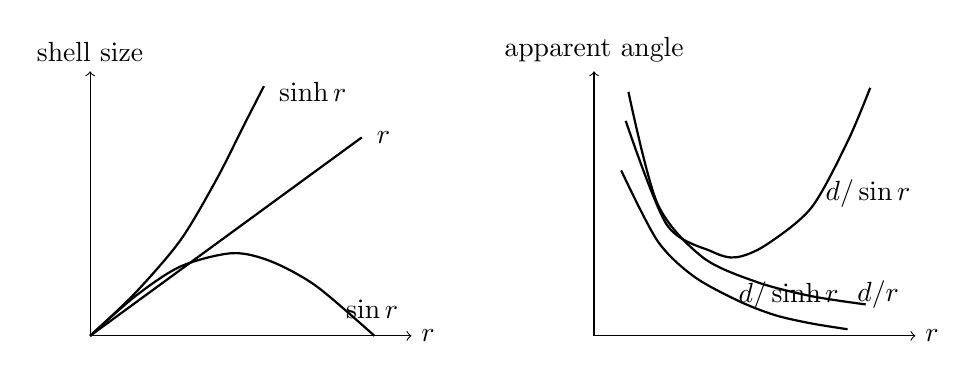
\begin{tikzpicture}[x=1.15cm,y=1.05cm]
\begin{scope}
\draw[->] (0,0)--(3.55,0) node[right] {$r$};
\draw[->] (0,0)--(0,3.2) node[above] {shell size};

\draw[thick] (0,0)--(3.0,2.4);
\draw (3.06,2.4) node[right] {$r$};

\draw[thick]
plot[smooth] coordinates {(0,0) (0.5,0.48) (1.0,0.84) (1.57,1.0) (2.0,0.9) (2.5,0.6) (3.14,0)};
\draw (2.72,0.55) node[below right] {$\sin r$};

\draw[thick]
plot[smooth] coordinates {(0,0) (0.5,0.52) (1.0,1.16) (1.4,1.9) (1.7,2.55) (1.92,3.02)};
\draw (1.98,2.95) node[right] {$\sinh r$};
\end{scope}

\begin{scope}[xshift=6.4cm]
\draw[->] (0,0)--(3.55,0) node[right] {$r$};
\draw[->] (0,0)--(0,3.2) node[above] {apparent angle};

\draw[thick]
plot[smooth] coordinates {(0.38,2.95) (0.7,1.6) (1.2,0.95) (1.8,0.65) (2.4,0.48) (3.0,0.38)};
\draw (2.8,0.5) node[right] {$d/r$};

\draw[thick]
plot[smooth] coordinates {(0.35,2.6) (0.8,1.35) (1.3,1.02) (1.57,0.95) (1.9,1.1) (2.4,1.55) (2.8,2.35) (3.05,3.0)};
\draw (2.45,1.72) node[right] {$d/\sin r$};

\draw[thick]
plot[smooth] coordinates {(0.3,2.0) (0.7,1.15) (1.1,0.72) (1.6,0.42) (2.0,0.25) (2.4,0.15) (2.8,0.08)};
\draw (2.15,0.2) node[above] {$d/\sinh r$};
\end{scope}
\end{tikzpicture}
\caption{Left: the shell-size factors \(r\), \(\sin r\), and \(\sinh r\), which control how many objects lie on a shell at distance \(r\). Right: the corresponding angular-size laws \(d/r\), \(d/\sin r\), and \(d/\sinh r\). On the sphere the apparent size turns around; in hyperbolic space it shrinks exponentially fast.}
\end{figure}

\subsection{Question \& Answer}

How could one tell that \(r\) is approaching \(\pi\) rather than simply becoming very large?

Because in the spherical discussion \(r\) is not an ordinary unbounded radial distance. It is an angular-distance coordinate on the unit sphere. Its range is finite:
\[
0 \le r \le \pi.
\]
So on the sphere ``large \(r\)'' means ``close to the antipode,'' not ``farther and farther without limit.'' If we later introduce a radius of curvature \(a\), we rescale the metric, but the unit variable \(r\) still runs only from \(0\) to \(\pi\).

\section{Stereographic Pictures and Hyperbolic Space}

Before introducing hyperbolic space, the lecture changes viewpoint again. It shows us a way of representing the sphere on the plane that is useful precisely because it distorts things. One rests the sphere on a plane tangent at the south pole and projects each point of the sphere to the plane by drawing the line from the north pole through that point. The north pole itself goes to infinity. Small circles near the south pole look small and almost undistorted; circles near the north pole blow up and look enormous on the plane.

That distortion is not a flaw in the sphere. It is a property of the projection. Intrinsically the sphere remains homogeneous. Equal intrinsic circles on the sphere map to circles of very different apparent sizes on the plane, but that does not mean the original geometry had special places.

\begin{figure}[htbp]
\centering
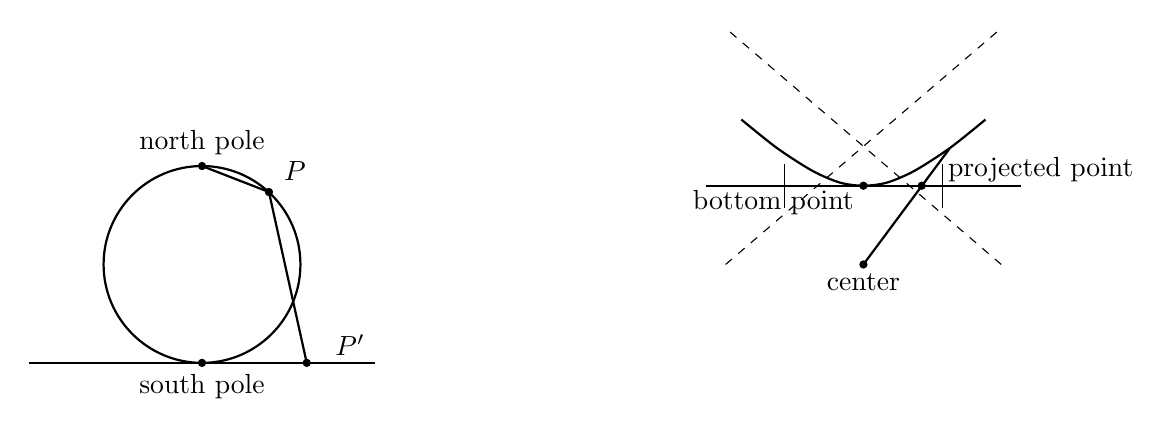
\begin{tikzpicture}[scale=1.0]
\begin{scope}[xshift=-4.2cm]
\draw[thick] (-2.2,-1.25)--(2.2,-1.25);
\draw[thick] (0,0) circle (1.25);
\fill (0,1.25) circle (1.5pt);
\fill (0,-1.25) circle (1.5pt);
\draw (0,1.55) node {north pole};
\draw (0,-1.55) node {south pole};

\fill (0.85,0.92) circle (1.5pt);
\draw (0.92,1.18) node[right] {$P$};
\draw[thick] (0,1.25)--(0.85,0.92)--(1.33,-1.25);
\fill (1.33,-1.25) circle (1.5pt);
\draw (1.57,-1.03) node[right] {$P'$};
\end{scope}

\begin{scope}[xshift=4.2cm]
\draw[thick] (-2.0,1)--(2.0,1);
\draw[dashed] (-1.75,0)--(1.75,3.0);
\draw[dashed] (1.75,0)--(-1.75,3.0);
\draw[thick]
plot[smooth] coordinates
{(-1.55,1.84) (-1.1,1.48) (-0.65,1.19) (-0.3,1.04) (0,1.0) (0.3,1.04) (0.65,1.19) (1.1,1.48) (1.55,1.84)};
\fill (0,0) circle (1.5pt);
\fill (0,1) circle (1.5pt);
\draw (0,-0.22) node {center};
\draw (0,0.78) node[left] {bottom point};
\draw[thick] (0,0)--(1.1,1.48);
\fill (0.74,1.0) circle (1.5pt);
\draw (0.95,1.2) node[right] {projected point};
\draw (-1,0.72) -- (-1,1.28);
\draw (1,0.72) -- (1,1.28);
\end{scope}
\end{tikzpicture}
\caption{Cross-sectional sketches of the two projection ideas used in the lecture: stereographic projection of the sphere onto a plane, and the analogous projection of the hyperboloid to a finite disk (shown here in cross-section as a finite interval).}
\end{figure}

Now the lecture brings in the third homogeneous geometry. In two dimensions the metric is
\begin{equation}
dh_2^2 = dr^2 + \sinh^2 r\, d\Omega_1^2,
\end{equation}
and in three dimensions,
\begin{equation}
dh_3^2 = dr^2 + \sinh^2 r\, d\Omega_2^2.
\end{equation}
Here \(r\) is reset once again. It is now the radial coordinate of hyperbolic space, and it runs from \(0\) to \(\infty\). The surrounding shells do not grow linearly, and they do not grow and then shrink. They grow like \(\sinh r\), and therefore they blow up exponentially fast.

To make that concrete, the lecture pauses to remind us that
\begin{equation}
\sin r = \frac{e^{ir}-e^{-ir}}{2i},
\qquad
\sinh r = \frac{e^r-e^{-r}}{2}.
\end{equation}
For large \(r\), the \(\sinh r\) factor is dominated by \(e^r/2\). That one fact is enough to explain both the geometry and the observation. The shells around us get very large very fast. Therefore the number of galaxies on a shell grows very fast. And therefore a fixed-size galaxy at fixed \(r\) subtends a very small angle. Explicitly,
\begin{equation}
d^2 = \sinh^2 r\, d\theta^2,
\qquad\text{so}\qquad
d\theta = \frac{d}{\sinh r}.
\end{equation}
At large \(r\),
\begin{equation}
d\theta \sim 2d\,e^{-r}.
\end{equation}
Thus hyperbolic space predicts the opposite observational signature from spherical space: distant objects look too small, and there are too many of them.

The lecture also gives a second model for this geometry, again as a visualization device. Introduce coordinates \(x\), \(y\), and \(T\), where \(T\) is \emph{not} physical cosmological time, and consider the surface
\begin{equation}
T^2 - x^2 - y^2 = 1.
\end{equation}
This is a hyperboloid. If the embedding space is given the Lorentz-signature metric
\begin{equation}
d\ell_{\mathrm{emb}}^2 = dT^2 - dx^2 - dy^2,
\end{equation}
then the induced geometry on the hyperboloid is homogeneous. The lecture phrases this in the language of Lorentz transformations: moving from one point of the hyperboloid to another is like tilting the time axis, and the induced geometry stays the same. Projecting the hyperboloid to the disk yields the Poincar\'e disk picture. No point ever reaches beyond the boundary circle; very distant points are crushed against it. Once again, that crushing is a property of the picture, not a failure of homogeneity.

\section{Radius of Curvature, Local Flatness, and the Torus Caveat}

Up to now we have mostly discussed unit geometries. The unit sphere has radius \(1\), and the unit hyperboloid is normalized similarly. But a real cosmological geometry comes with a radius of curvature. The lecture denotes it by a little \(a\). If all lengths are scaled by \(a\), then squared lengths are scaled by \(a^2\). Therefore the metric of a radius-\(a\) sphere is obtained by multiplying the unit metric by \(a^2\):
\begin{equation}
ds^2 = a^2 d\Omega_n^2.
\end{equation}
Likewise, for hyperbolic space,
\begin{equation}
ds^2 = a^2 dh_n^2.
\end{equation}
In explicit radial form this is
\begin{align}
ds_{\mathrm{sphere}}^2 &= a^2\left(dr^2 + \sin^2 r\, d\Omega_{n-1}^2\right),\\
ds_{\mathrm{hyp}}^2 &= a^2\left(dr^2 + \sinh^2 r\, d\Omega_{n-1}^2\right).
\end{align}
The lecture explicitly asks why the factor is \(a^2\) rather than \(a\), and the answer is simply that the metric measures squared distance.

This is also where the lecture ties geometry back to observation. If \(a\) is very large, then over distances small compared with \(a\) all three geometries look nearly flat. That is why local observations cannot distinguish them if the radius of curvature is huge. A basketball looks more curved than the Earth's surface because its radius is smaller. Increasing the size of the geometry decreases its curvature. In the lecture's observational summary, flatness to about the one-percent level is translated into the statement that the universe must be at least about ten times larger in radius than the visible region if it is not exactly flat.

\subsection{Question \& Answer}

Can a universe be flat and still finite?

Yes. This is the lecture's explicit correction to its own earlier simplification. The three constant-curvature simply connected cases are not the whole story. One may have a flat geometry with nontrivial topology, and the torus is the standard example.

The mathematically clean definition does not begin with a donut embedded in three-space. It begins with a rectangle in the plane. Identify the left and right edges pointwise. Identify the top and bottom edges pointwise. Then walking out through one side of the rectangle brings you back through the opposite side. Locally the geometry is just the flat geometry of the rectangle; globally the space is periodic.

\begin{figure}[htbp]
\centering
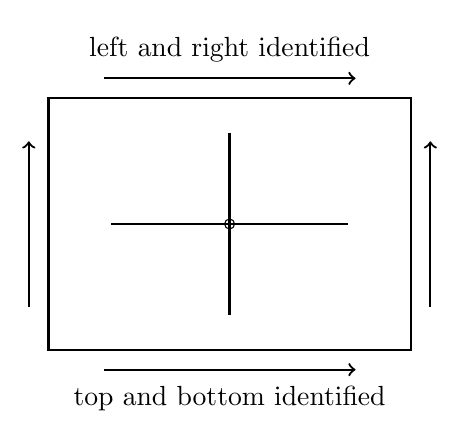
\begin{tikzpicture}[scale=1.0]
\draw[thick] (0,0) rectangle (4.6,3.2);

\draw[->,thick] (0.7,3.45)--(3.9,3.45);
\draw[->,thick] (0.7,-0.25)--(3.9,-0.25);

\draw[->,thick] (-0.25,0.55)--(-0.25,2.65);
\draw[->,thick] (4.85,0.55)--(4.85,2.65);

\draw[thick] (0.8,1.6)--(3.8,1.6);
\draw[thick] (2.3,0.45)--(2.3,2.75);

\draw (2.3,1.6) circle (1.8pt);

\draw (2.3,-0.62) node {top and bottom identified};
\draw (2.3,3.82) node {left and right identified};
\end{tikzpicture}
\caption{A torus described as a rectangle with opposite sides identified. Locally the geometry is flat; globally it is periodic.}
\end{figure}

This also explains what would be observed if the torus were small enough. A toroidal universe is equivalent to flat space filled with periodic copies of everything. One would see repeated images of the same objects, and in the extreme case one would see repeated images of oneself. If the fundamental cell were large enough, however, the periodicity could remain unnoticed. So yes: a universe may be finite and flat, provided the finiteness is topological rather than the result of positive curvature.

\section{From Spatial Geometry to Spacetime Cosmology}

Only after the static spatial story is in place does the lecture turn to spacetime. We begin with special relativity. Setting the speed of light equal to \(1\), Minkowski space has metric
\begin{equation}
ds^2 = -dt^2 + dx^2 + dy^2 + dz^2.
\end{equation}
The time contribution has the opposite sign from the spatial ones. A light ray is a null ray, meaning that
\begin{equation}
ds^2 = 0.
\end{equation}
If the light ray moves only along the \(x\)-axis, then
\begin{equation}
-dt^2 + dx^2 = 0
\qquad\Rightarrow\qquad
dx = \pm dt.
\end{equation}
So light travels at unit speed to the left or to the right.

Now comes the cosmological deformation. Keep the time term \(-dt^2\), but replace the flat spatial metric by one of the homogeneous metrics we have just built. Then let the overall spatial size vary with time. The lecture writes this scale factor as \(A(t)\); we will write it as \(a(t)\) to distinguish it clearly from the fixed curvature radius \(a\) of the preceding static discussion.

For visualization the lecture first uses a \(2+1\)-dimensional toy model:
\begin{equation}
ds^2 = -dt^2 + a(t)^2 d\Omega_2^2.
\end{equation}
This is a world with one time dimension and a spatial geometry that is a two-sphere whose radius changes with time. The same construction in \(3+1\) dimensions is written more economically as
\begin{equation}
ds^2 = -dt^2 + a(t)^2 d\Sigma^2,
\end{equation}
where \(d\Sigma^2\) is one of the three spatial metrics:
\begin{align}
d\Sigma^2 &= dx^2 + dy^2 + dz^2,\\
d\Sigma^2 &= d\Omega_3^2,\\
d\Sigma^2 &= dh_3^2.
\end{align}
Thus the three cosmological metrics of interest are
\begin{align}
ds^2 &= -dt^2 + a(t)^2 \left(dx^2+dy^2+dz^2\right),\\
ds^2 &= -dt^2 + a(t)^2 d\Omega_3^2,\\
ds^2 &= -dt^2 + a(t)^2 dh_3^2.
\end{align}

The lecture then recovers the Hubble law kinematically. Take two points whose angular separation \(\theta\) is fixed in the comoving coordinates. Their actual separation is
\begin{equation}
D = a(t)\theta.
\end{equation}
Differentiate with respect to time while keeping \(\theta\) fixed:
\begin{equation}
V = \dot a(t)\theta.
\end{equation}
Eliminating \(\theta\) yields
\begin{equation}
V = \frac{\dot a}{a} D.
\end{equation}
So the Hubble parameter is
\begin{equation}
H = \frac{\dot a}{a}.
\end{equation}
This derivation does not depend on whether the spatial geometry is flat, spherical, or hyperbolic. What matters is that all comoving distances are multiplied by the same scale factor.

At this point geometry gives way to dynamics. Once the cosmological metric has been reduced to a single unknown function \(a(t)\), the next question is: what equation determines \(a(t)\)? The lecture stops at exactly this threshold. The answer, to be taken up next, comes from general relativity and leads to the Friedmann equations.

\section{Summary}

The lecture unfolds in a very deliberate sequence. First we stop treating flatness as a principle and ask instead which non-flat spaces remain possible once homogeneity is imposed. Then we move into the metric language, beginning with flat space and its polar form, and we isolate \(d\Omega_1^2\) as the metric of the unit circle. From there we build the sphere by replacing the flat shell factor \(r^2\) with \(\sin^2 r\), and the same pattern immediately produces the \(3\)-sphere. Once the spherical metrics are in hand, the lecture turns to observation: angular sizes and galaxy counts reveal that positively curved space makes distant objects look too large and distant shells contain too few galaxies. Stereographic projection then prepares the way for hyperbolic space, where the shell factor is \(\sinh^2 r\), distant objects look too small, and the number of distant objects grows too quickly. After introducing the radius of curvature and the fact of local flatness, the lecture corrects its own earlier oversimplification by adding the torus as a flat but finite topological possibility. Only then does time return. Minkowski space is recalled, a time-dependent scale factor is inserted into the spatial metric, the Hubble law is recovered kinematically, and the chapter ends exactly where the lecture ends: with the promise of Friedmann dynamics.